\chapter{Zahlenfolgen, Zahlenreihen, Konvergenz}

Der moderne Grenzwertbegriff stellt die Grundlage der Infinitesimalrechnung dar. In diesem Kapitel betrachten wir zuerst Zahlenfolgen und Reihen, definieren dann Konvergenz sowie Grenzwert und lernen abschließend
einige wichtige Regeln zur Konvergenz und Grenzwertbestimmung kennen.

Um die Wichtigkeit zu illustrieren, warum eine exakte Definition der Konvergenz notwendig ist, sei Zenons Paradoxon von Achilles und der Schildkröte angeführt. \emph{Zeno of Elea} (etwa 500 BC) hat dieses Paradoxon angeführt, um zu zeigen, dass der naive Begriff von Wandel und Bewegung nur eine Illusion wäre. Zur besseren Veranschaulichung wählen für die folgende Erklärung (willkürlich gewählte) Größenabgaben. In dem Paradox nun veranstalten Achilles und eine Schildkröte ein Wettrennen, wie in Abbildung \ref{fig:ZenoAchilles} dargestellt. Achilles ist in der Lage, mit einer Geschwindigkeit von $25\ukmh$ zu rennen, während die Schildkröte nur $5\ukmh$ schafft. Der Fairness halber erhält die Schildkröte daher einen Vorsprung von $100\ukm$. Die Frage ist nun, wann Achilles die Schildkröte überholt. Der geläufige physikalische Ansatz wäre, ein Koordinatensystem zu definieren, die Bewegungsgleichungen beider Partizipanten aufzustellen und den Schnittpunkt zu berechnen. Zenon argumentiert allerdings wie folgt:

\begin{enumerate}
	\item Damit Achilles die Schildkröte überholen kann, muss er zunächst den Vorsprung von $100\ukm$ aufholen. Dazu benötigt er $4$ Stunden.
	\item In diesen $4$ Stunden allerdings ist die Schildkröte bereits $20\ukm$ weiter gekrochen.
	\item Also muss Achillles im nächsten Schritt diese $20\ukm$ Vorsprung aufholen, wozu er $0.8$ Stunden benötigt. Aber nun hat die Schildkröte bereits einen neuen Vorsprung erhalten.
	\item Egal, wie oft Achilles also den Vorsprung aufholt, um die Schildkröte zu überholen, müsste er unendliche viele Vorsprünge aufholen. Also holt Achilles die Schildkröte nie ein, um kann sie somit auch nicht überholen.
\end{enumerate}

Wie lässt sich dieses Paradoxon auflösen? Der Fehler, den Zenon hier begeht, besteht darin, dass Achilles zum Aufholen "unendlicher" vieler Vorsprünge auch "unendlich" viel Zeit benötigt. Dies ist aber bei einer genauen Betrachtung mithilfe eines exakten Grenzwertbegriffs nicht der Fall, wie wir auch in einer Übungsaufgabe nachweisen werden.

\begin{figure}[H]
	\caption{Zenos Paradoxon von dem Wettrennen zwischen Achilles und der Schildkröte}
	\label{fig:ZenoAchilles}
	\centering
	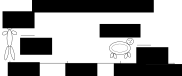
\includegraphics[width=0.95\textwidth]{./svg/zeno-achilles.png}
\end{figure}

\section{Zahlenfolgen}

Bevor wir den Begriff der Konvergenz näher definieren können, benötigen wir zuerst ein Verständnis von Zahlenfolgen.

\begin{definition}{Unendliche Zahlenfolge}{UnlimitSeq}
	Eine unendliche Zahlenfolge ist gegeben, wenn jeder natürlichen Zahl $n \ge 0$  genau eine (meist reelle) Zahl $a_n\in\R$ zugeordnet wird. $a_n$ heißt das $(n+1)$-te Glied der Zahlenfolge.
\end{definition}

\begin{definition}{Endliche Zahlenfolge}{LimitSeq}
	Besteht die Zuordnung nur für jede natürliche Zahl $n$ zwischen 0 und $N$ ($0 \ge n \ge N$), so spricht man von einer endlichen Zahlenfolge.
\end{definition}

Zahlenfolgen können also als Funktion $f: \N \to \R$ aufgefasst werden. Zur mathematischen Darstellung gibt es zwei Möglichkeiten:

\begin{enumerate}
	\item Explizite Darstellung: Der Wert des $n$.-ten Folgenglieds ist direkt gegeben. 
	\item Implizite (rekursive) Darstellung: Der Wert des nächsten Folgengliedes ($n+1$) ist gegeben in Abhängigkeit eines oder mehrerer voriger Folgenglieder. Zudem ist ein Startwert für das erste oder die ersten Folgenglieder gegeben.
\end{enumerate}

Wir wollen uns diese beiden Möglichkeiten an zwei wichtigen Zahlenfolgen anschauen.

\begin{definition}{Arithmetische Zahlenfolge}{ArithSeq}
	Eine arithmetische Zahlenfolge ist gegeben, wenn in jedem Schritt das nächste Folgenglied durch Addition einer immer gleichen Konstanten zum vorigen Folgenglied bestimmt wird.
\end{definition}

\begin{definition}{Geometrische Zahlenfolge}{GeoSeq}
	Eine geometrische Zahlenfolge ist gegeben, wenn in jedem Schritt das nächste Folgenglied durch Multiplikation einer immer gleichen Konstanten mit dem vorigen Folgenglied bestimmt wird.
\end{definition}

Eine arithmetische Zahlenfolge beschreibt konstantes Wachstum und kann auch als lineare Funktion aufgefasst werden. Demgegenüber drückt eine geometrische Zahlenfolge exponentielles Wachstum, etwa die (initiale) Vermehrung von Bakterien in einer Petrischale. In Beispiel \ref{ex:ArithSeq} und \ref{ex:GeoSeq} sind diese beiden Zahlenfolgen anhand eines konkreten Beispiels in beiden Darstellungsformen zu sehen.

\begin{example}{Darstellung einer arithmetischen Zahlenfolge}{ArithSeq}
	Die arithmetische Zahlenfolge der ungeraden Zahlen beginnt mit $(a_n) = 1, 3, 5, 7, 9, ...$. Das Zahlenfolgenglied für $n=0$ ist $a_0=1$. Für $n=1$ ist $a_1=3$, für $n=2$ ist $a_2=5$. Wir erkennen sofort,
dass ein Folgenglied immer um $2$ größer ist als das vorige. Die rekursive Darstellung lautet somit also $a_{n+1} = a_n + 2$ mit dem Startwert $a_0 = 1$.  Wenn wir es nun noch schaffen, eine Formel für $a_n$ in Abhängigkeit von $n$ zu finden, haben wir auch die explizite Darstellung gefunden: $a_n = 2n+1$.
\end{example}

\begin{example}{Darstellung einer geometrischen Zahlenfolge}{GeoSeq}
	Analoges gilt für die geometrischen Zahlenfolgen. Beispielsweise ist $(a_n) = 1, \frac{1}{2}, \frac{1}{4}, \frac{1}{8}, \frac{1}{16}, ...$ eine geometrische Zahlenfolge. Jedes Folgenglied ergibt sich, indem das
vorige Folgenglied halbiert wird. Damit können wir die rekursive Darstellung angeben als $a_{n+1} = \frac{1}{2}a_n$ mit dem Startwert $a_0=1$. Für die explizite Darstellung erhalten wir nach etwas Nachdenken $a_n = {\frac{1}{2}}^n$. Wichtig zu betonen ist hier, dass es keine allgemein gültige Vorgehensweise gibt, die rekursive Darstellung in die explizite Darstellung umzuwandeln, hier ist wie in vielen Teilen der Mathematik kreatives Nachdenken erforderlich.
\end{example}

\begin{figure}[p]
	\caption{Graphische Darstellung der arithmetischen Folge aus \ref{ex:ArithSeq}}
	\label{fig:ExArithSeq}
	\centering
	\includegraphics[width=0.8\textwidth]{./gnuplot/example-arithmetic-series.png}
\end{figure}

\begin{figure}[p]
	\caption{Graphische Darstellung der geometrischen Folge aus \ref{ex:GeoSeq}}
	\label{fig:ExGeoSeq}
	\centering
	\includegraphics[width=0.8\textwidth]{./gnuplot/example-geometric-series.png}
\end{figure}

Wie in Abbildung \ref{fig:ExArithSeq} und \ref{fig:ExGeoSeq} dargestellt, lässt sich eine Zahlenfolge auch in einem Diagramm darzustellen. Hierbei ist zu beachten, dass nur Punkte, aber keine durchgehenden Linien eingezeichnet werden dürfen - denn der Definitionsbereich besteht nur aus den natürlichen Zahlen. Ebenfalls diesen beiden Abbildungen lässt sich entnehmen, dass Zahlenfolgen unterschiedlich verlaufen können. Die arithmetische Reihe steigt ohne Grenzen an, die geometrische Reihe $(a_n) = (\frac{1}{2})^n$ fällt und nähert sich immer weiter der $0$ an. Dies gibt Anlass, zwei wichtige Eigenschaften von Zahlenfolgen zu definieren.

\begin{definition}{Monotonie einer Zahlenfolge}{MonoSeq}
	Eine Zahlenfolge $(a_n)$ heißt \textbf{streng monoton wachsend}, wenn jedes Glied größer ist als das vorige, also $\forall n \in\N: a_{n+1} > a_n$ gilt. Analog heißt die Zahlenfolge \textbf{streng monoton fallend}, wenn jedes Glied kleiner ist als das vorige, also $\forall n \in\N: a_{n+1} < a_n$ gilt. Gilt nur $a_{n+1} \ge a_n$ beziehungsweise $a_{n+1} \le a_n$, so spricht man nur von einer \textbf{monoton steigenden} beziehungsweise \textbf{monoton fallenden} Folge (ohne dem Wörtchen "streng").
\end{definition}

\begin{definition}{Beschränktheit einer Zahlenfolge}{BoundSeq}
	Eine Zahlenfolge $(a_n)$ heißt \textbf{nach unten beschränkt}, wenn alle ihre Glieder überhalb einer unteren Grenze liegen, das heißt, wenn es ein $L\in\R$ gibt, sodass $\forall n \in\N: L \ge a_n$ gilt. $L$ heißt dann untere Schranke (lower bound) der Zahlenfolge, geschrieben als $L = \inf a_n$ (Infimum).
	
	Eine Zahlenfolge $(a_n)$ heißt \textbf{nach oben beschränkt}, wenn alle ihre Glieder unterhalb einer oberen Grenze liegen, das heißt, wenn es ein $U\in\R$ gibt, sodass $\forall n \in\N: L \le a_n$ gilt. $L$ heißt dann obere Schranke (lower bound) der Zahlenfolge, geschrieben als $U = \sup a_n$ (Supremum).
\end{definition}

Anmerkung: Manchmal betrachtet man auch nur die Beschränktheit einer Zahlenfolge ohne die ersten $N$ Glieder und schreibt dann $\inf\limits_{n \ge N} a_n$ beziehungsweise $\sup\limits_{n \ge N} a_n$.

\begin{example}{Eigenschaften der arithmetischen und geometrischen Zahlenfolge}{ArithGeoProp}
	Die arithmetische Zahlenfolge $a_{n+1} = a_n + C, a_0 = k, C > 0$ ist streng monoton steigend, denn $a_{n+1} > a_n$ ist äquivalent zu $a_n + C > a_n$ und weiter $C > 0$, was nach Voraussetzung eine wahre Aussage ist. Weiterhin ist sie nicht nach oben beschränkt (\textbf{unbeschränkt}), da für jede noch so große Zahl $U > 0$ sich durch Umstellung der expliziten Darstellung ein Folgenglied $n'$ finden lässt, sodass $a_{n'} > U$ gilt. Allerdings ist sie nach unten beschränkt, dass alle Glieder größer oder gleich dem Startwert $k$ sind.
	
	Analog findet man für arithmetische Zahlenfolgen mit $C<0$, dass sie monoton fallend, nach oben beschränkt und nach unten unbeschränkt ist. Für $C=0$ erhält man die sogenannte konstante Folge, welche sowohl mononton steigend als auch fallend ist (aber nicht streng), und sowohl nach oben als auch nach unten beschränkt ist.
	
	Für die geometrische Zahlenfolge $a_{n+1} = q \cdot a_n, a_0 = p, 0 < q < 1, p > 0$ stellt wir zuerst fest, dass alle ihre Glieder positiv sind. Sie ist streng monoton fallend, denn $a_{n+1} < a_n$ ist äquivalent zu $q \cdot a_n < a_n$ und weiter (da $a_n$ positiv) $q < 1$, was nach Voraussetzung eine wahre Aussage ist. Sie ist nach oben beschränkt, da sie monoton fallend ist. Weiterhin ist sie auch nach unten beschränkt, da alle Folgeglieder positiv sind (und damit $L=0$ eine untere Schranke darstellt).	
\end{example}

\section{Konvergenz und Grenzwertbegriff}

Eine weitere Eigenschaft von fundamentaler Bedeutung ist das sogenannte Konvergenzverhalten einer Zahlenfolge. An dem Beispiel der geometrischen Folge $(\frac{1}{2})^n$ in Abbildung \ref{fig:ExGeoSeq} haben wir bereits gesehen, dass sich diese scheinbar immer weiter der $0$ anzunähern scheint, ohne diese jemals (im Endlichen) zu erreichen. Diese Idee, dass eine Folge sich einem Grenzwert immer weiter nähert, wird durch die folgende Definition präzisiert.

\begin{definition}{Konvergenz und Grenzwert}{Convergence}
	Eine Folge $(a_n)$ heißt \textbf{konvergent} mit dem \textbf{Grenzwert} $\alpha$, wenn der Abstand der Folgenglieder zum Grenzwert beliebig klein wird und klein bleibt. Andernfalls heißt sie \textbf{divergent}.
	
	$\forall \epsilon > 0 \exists n_0\in\N: \forall n > n_0 : |a_n - \alpha| < \epsilon$
	
	Man schreibt dann: $\lim\limits_{n\to\infty} a_n = \alpha$.
\end{definition}

Anders formuliert kann man auch sagen, die Folge $(a_n)$ heißt konvergent mit dem Grenzwert $\alpha$, wenn man zu jedem noch so kleinen Abstand zum Grenzwert (bezeichnet mit $\epsilon$) immer eine Position in der Zahlenfolge finden kann, sodass alle Folgenglieder rechts von dieser Position innerhalb dieses Abstands liegen. Visuell wird diese Definition durch Abbildung \ref{fig:VisLimit} illustriert.

\begin{figure}[h]
	\caption{Graphische Veranschaulichung des Grenzwertbegriffs}
	\label{fig:VisLimit}
	\centering
	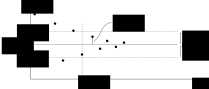
\includegraphics[width=0.8\textwidth]{./svg/definition-convergence.png}
\end{figure}

In Beispiel \ref{ex:ConvGeoSeq} und \ref{ex:ConvConstSeq} wird gezeigt, wie man anhand dieser Definition nachweisen kann, ob eine Folge konvergent ist und welchen Grenzwert sie hat. Ebenfalls wie in Beispiel \ref{ex:ConvAltSeq} kann man zeigen, dass eine Folge divergent ist. Für die praktische Bestimmung von Grenzwerten ist diese Definition sehr umständlich, wir werden daher in Kürze Rechenregeln kennen lernen, um die Berechnung von Grenzwerten zu vereinfachen.

\begin{example}{Konvergenz der geometrischen Folge}{ConvGeoSeq}
	Wir betrachten noch einmal die geometrische Folge $a_n = (\frac{1}{2})^n$. Wir vermuten, dass $\alpha=0$ der Grenzwert ist. Um dies zu beweisen, benutzen wir die obige Definition. Sei $\epsilon>0$. Wir müssen
	nun ein $n_0$ finden, sodass $|a_n-\alpha|=(\frac{1}{2})^n < \epsilon$ gilt, wenn $n > n_0$. Durch Umstellen der Ungleichung erhalten wir $n > \log_{1/2}(\epsilon)$ (man beachte, dass sich das Ungleichheitszeichen umkehrt, da $\log_{1/2}$ eine monoton fallende Abbildung ist). Die Ungleichung ist also erfüllt, solange wir Folgenglieder $a_n$ betrachten, wo $n$ größer als $\log_{1/2}(\epsilon)$ ist. Abschließend setzen wir $n_0 = \floor{\log_{1/2}(\epsilon)}$, wobei die Klammer mit dem unteren Hacken für die Operation "Abrunden" stehen. Damit können wir schreiben:

	$$
	\forall \epsilon > 0 \exists n_0 = \floor{\log_{1/2}(\epsilon)} : \forall n > n_0 : |a_n - 0| < \epsilon
	$$
		
	Also ist die geometrische Folge $a_n = (\frac{1}{2})^n$ konvergent und hat den Grenzwert $\alpha=\lim\limits_{n\to\infty}(\frac{1}{2})^n=0$.
\end{example}


\begin{example}{Konvergenz der konstanten Folge}{ConvConstSeq}
	Die konstante Folge $a_n = 1$ ist ebenfalls konvergent und hat den Grenzwert $\alpha = 1$, denn für den Abstand gilt $|a_n-\alpha|=|1-1|=0<\epsilon$. Wir erkennen an diesem Beispiel, dass es nicht von Relevant ist, ob die Folgenglieder den Grenzwert erreichen oder nicht -- entscheidend ist lediglich der Abstand zum Grenzwert, und dieser kann auch $0$ betragen kann.
\end{example}


\begin{example}{Divergenz der alternierenden Folge}{ConvAltSeq}
	Die Folge $a_n = (-1)^n$ mit den Gliedern $1,-1,1,-1,...$ heißt alternierende Folge. Diese ist zwar nach oben und unten beschränkt (durch $L=-1$ und $U=1$), besitzt allerdings keinen Grenzwert. Wählt man etwa $\alpha=1$, erhält man für den Abstand $(d_n) = |a_n-\alpha|=(-1)^n-1| = (0, 2, 0, 2, 0, 2)$. Ist $\epsilon$ nun genügend klein, etwa $0.5$, so findet man immer wieder ein Folgenglied, dessen Abstand zum Grenzwert größer ist als $\epsilon$. Egal, welchen Grenzwertkandidaten man wählt, es ist nicht möglich, den Abstand zum Grenzwertkandidaten beliebig klein zu halten.  
\end{example}

Ist eine Folge nicht konvergent, so heißt Sie wie erwähnt divergent und besitzt folglich auch keinen Grenzwert. Nun gibt es eine besondere Art der Divergenz, bei der man gelegentlich auch davon spricht, der Grenzwert sei $\pm\infty$. Diese Aussage ist immer im Sinne der folgenden Definition zu verstehen:

\begin{definition}{Bestimmte Divergenz}{Divergence}
	Eine Folge heißt \textbf{bestimmt divergent} gegen $+\infty$ ($-\infty$), falls die Folgenglieder beliebig groß (klein) werden und auch groß (klein) bleiben.

	$$
	\forall R > 0 \exists n_0\in\N: \forall n > n_0 : a_n > R
	$$
	
	$$
	\forall R < 0 \exists n_0\in\N: \forall n > n_0 : a_n < R
	$$

	Man schreibt dann auch $\lim\limits_{n\to\infty}a_n = +\infty$ beziehungsweise $\lim\limits_{n\to\infty}a_n = -\infty$.
\end{definition}


\begin{example}{Divergenz der arithmetischen Folge}{DivArithSeq}
	Die arithmetische Folge $a_n=2n+1$ ist bestimmt divergent gegen $\infty$. Aus $2n+1 > R$ erhalten wir $n > \frac{R-1}{2}$ Wählen wir nun $n_0 = \floor{\frac{R-1}{2}}$, so können wir schreiben:
	
	$$
	\forall R > 0 \exists n_0 = \floor{\frac{R-1}{2}}: \forall n > n_0 : a_n > R
	$$
		
	Es ist also $\lim\limits_{n\to\infty} 2n+1 = \infty$.
\end{example}


\section{Reihe}

Bei einer Reihe handelt es sich um eine ganz bestimmte Form einer Zahlenfolge, die eine eigene Bezeichnung erhalten hat, das sie in der Praxis häufig vorkommt.

\begin{definition}{Begriff der Reihe}{Series}
	Eine \textbf{Reihe} $(s_n)$ entsteht durch Summation der Glieder einer Zahlenfolge. Die Summe $s_n=\sum\limits_{i=0}^n a_i$ der ersten $(n+1)$-Glieder heißt \textbf{Partialsumme}. Der Grenzwert der Partialsummen $s_\infty = \lim\limits_{n\to\infty}s_n$ heißt \textbf{unendliche Reihe}.
\end{definition}


Beispiel arith / geometr. Reihe

\section{Konvergenz von Folgen}

Spezielle Grenzwerte

Grenzwertsätze, a+-b, a*/b, f(a_n), lhospital

\section{Konvergenz von Reihen}

Nullfolge

Quotienten und Wurzelkriterium
